\section{Internet of Things} % (fold)
\label{sec:internet_of_things}
Som en del af løsningen skal der indgå en sensorer, der kan detektere både i havnen. For at finde ud af mere, om hvad der er muligt, er konceptet \enquote{Internet of Things}, herefter IoT, blevet undersøgt. IoT er et paradigme, hvor alle fysiske genstande skal være unikt identificerbare, således at computere nemmere kan administrere disse genstande. Derudover handler IoT om at forbinde disse genstande i et netværk \cite{kopetz2011real}. En mere beskrivende definition af IoT er derfor \enquote{a world-wide network of interconnected objects uniquely addressable, based on standard communication protocols} \cite{iot_survey_2010}.

\subsection{Konceptet}
\label{sub:iot_koncept}
IoT er ofte beskrevet ud fra forskellige visioner for paradigmet. I \cite{iot_survey_2010}  beskrives tre visioner; \enquote{Things oriented}, \enquote{Internet oriented} og \enquote{Semantic oriented}. Disse visioner er opstået ud fra de forskellige interessenter i IoT. Disse interessenter angriber IoT fra forskellige vinkler og er derfor kommet fra til forskellige definitioner af IoT. Se \cref{fig:iot_visions}.

Den første definition af IoT, \enquote{Things oriented}, stammer fra Auto-ID labs, et verdensomspændende netværk af forskere indenfor Radio Frequency IDentification (RFID) og anden sensor teknologi. Målet med IoT er i denne definition at forbedre synligheden og muligheden for at spore genstande. For at opnå dette er Electronic Product Code (EPC) standarden blevet udviklet. Denne standard har til formål at sprede brugen af RFID samt andre teknologier \cite{iot_survey_2010}.

Den anden vision for IoT, \enquote{Internet oriented}, bygger videre på den første definition. Denne vision består i, at alle objekter selv kan forbinde sig til hinanden og computere. Konsortiummet CASAGRAS har fokus på at skabe \enquote{a world where things can automatically communicate to computers and each other, providing services to the benefit of the human kind} \cite{iot_survey_2010}.

Den sidste vision der beskrives her, \enquote{Semantic oriented}, omhandler hvordan de data, der genereres i \enquote{Things oriented} delen af IoT, organiseres. Visionen behandler strukturering af store mængder data, med hensigten at der opnås en forbedret overskuelighed og menneskelig forståelse, af disse ellers ofte overvældende mængder data \cite{iot_semantics_2012}.


\begin{figure}
  \centering
  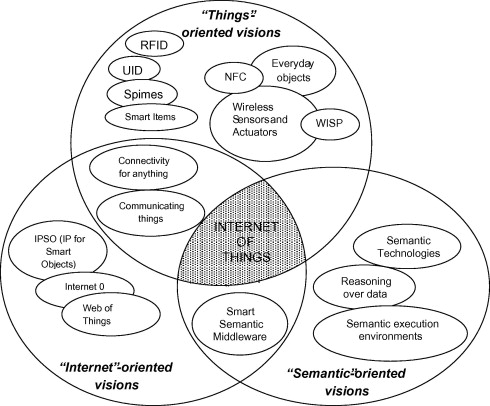
\includegraphics[width=\textwidth]{iot_visions}
  \caption{Internet of Things paradigmet ud fra tre visioner. Fra \cite{iot_survey_2010}.}
  \label{fig:iot_visions}
\end{figure}

\subsection{RFID}
RFID står for Radio Frequency IDentification, og som navnet antyder kan teknologien identificere objekter ved hjælp af radio frekvenser. Et RFID-tag, er en lille chip der indeholder en antenne, og en lille mængde data. Et objekt med et RFID-tag er nu \enquote{tagget}, og data om objektet kan læses ved hjælp af en RFID læser. Man kategoriserer typisk RFID-tags i passive og aktive. Et aktivt RFID-tag kræver strøm for at blive læst, og er derfor ofte tilsluttet et batteri. Et passivt RFID-tag kræver ingen strøm fra et batteri, men får derimod strømmen fra RFID-læseren \cite{want2006rfid}.

\subsection{Anvendelse af Internet of Things på Vestre Bådehavn}
\label{sub:iot_vestre_baadehavn}

Som beskrevet i \cref{sub:iot_koncept}, er der mange muligheder for hvilke sensorer der kan benyttes til at identificere objekter. Dette afsnit vil se på RFID og ultralyds sensorer, samt kameraer med billedgenkendelses software, som mulige sensorer, der kan benyttes på en havn som Vestre Bådehavn.

Lad os antage at alle både er blevet tagget med passive RFID-tags, sådan at de hver har en unik identifikation. Passive RFID-tags vægles da de er billige, og kan sidde på både uden nogen direkte afhængighed af elektricitet. Derudover kan hver vandlejeplads registrere, ved hjælp af en sensor, hvorvidt vandlejepladsen er optaget. Hvis der ligger en båd, kan en anden sensor også se hvem der ejer båden.

Sensoren som registrerer hvorvidt der ligger en båd på en vandlejeplads, kunne være en ultralyds sensor. Denne kan ved hjælp af lydbølger detektere tilstedeværelse af et objekt. Den kan dog ikke med stor præcision identificere objektet. En anden løsning er et kamera der ved hjælp af billed genkendelse kan identificere båden.

En computer forbundet til disse to typer sensorer, kan nu effektivt administrere en kæmpe havn med mange vandlejepladser. Når en ny båd lægger til på en vandlejeplads, vil computeren med det samme vide dette. Computeren kan derudover også kategorisere båden som en medlemsbåd eller som en gæstebåd. Da computeren nu har registreret at vandlejepladsen er optaget, skal den vende et skilt eller tænde for en diode, eller på anden måde ændres pladsens status til optaget.


\subsection{Opsummering}

I dette projekt arbejdes der udelukkende på en software løsning, og ikke på implementering af hardware. Derfor vil sensorerne som skal registrere bådene i havnen, blot blive simuleret, da deres tekniske opbygning ikke er direkte relevant for implementeringen af software løsningen. 

De simulerede sensorer kan opfatte tre tilstande. Enten kan den registrere at der ligger en ukendt båd, en kendt båd, eller ingen båd. Den ukendte båd vil være en gæst, og den kendte båd et medlem. Når en sensor opfanger et skift fra én tilstand til en anden, vil den sende et signal til softwareløsningen med info om den nye tilstand.

Det vurderes, på baggrund at den stigende interesse for \enquote{Internet of Things}, at denne slags sensorer er en del af en realistisk fremtidshorisont. Dette er en væsentlig forudsætning for den følgende løsningsmodels udgangspunkt.
